\documentclass{article}
\newcommand{\ii}{{\bf i}}
\newcommand{\jj}{{\bf j}}
\newcommand{\kk}{{\bf k}}
\newcommand{\id}{{\bf 1}}
\newcommand{\hur}{\frac{\id+\ii+\jj+\kk}{2}}%The "Hurwitz point"
\newcommand{\hurwitz}{\Z\left[\hur,\ii,\jj,\kk\right]}%The set of Hurwitz integers
\usepackage[utf8]{inputenc}
\usepackage[dvips]{graphicx}
\usepackage{a4wide}
\usepackage{amsmath}
\usepackage{euscript}
\usepackage{amssymb}
\usepackage{amsthm}
\usepackage{amsopn}
\usepackage[colorinlistoftodos]{todonotes}
\usepackage{graphicx}
\usepackage[T1]{fontenc}
\newcommand\mybar{\kern1pt\rule[-\dp\strutbox]{.8pt}{\baselineskip}\kern1pt}

\usepackage{ulem}
\usepackage{xcolor}
\newcommand{\cs}[1]{\color{blue}{#1}\normalcolor}

%Matrix commands
\newcommand{\ba}{\begin{array}}
\newcommand{\ea}{\end{array}}
\newcommand{\bmat}{\left[\begin{array}}
\newcommand{\emat}{\end{array}\right]}
\newcommand{\bdet}{\left|\begin{array}}
\newcommand{\edet}{\end{array}\right|}

%Environment commands
\newcommand{\be}{\begin{enumerate}}
\newcommand{\ee}{\end{enumerate}}
\newcommand{\bi}{\begin{itemize}}
\newcommand{\ei}{\end{itemize}}
\newcommand{\bt}{\begin{thm}}
\newcommand{\et}{\end{thm}}
\newcommand{\bp}{\begin{proof}}
\newcommand{\ep}{\end{proof}}
\newcommand{\bprop}{\begin{prop}}
\newcommand{\eprop}{\end{prop}}
\newcommand{\bl}{\begin{lemma}}
\newcommand{\el}{\end{lemma}}
\newcommand{\bc}{\begin{cor}}
\newcommand{\ec}{\end{cor}}
\newcommand{\lcm}{\mbox{lcm}}
\newcommand{\defn}{\fbox{definition}}
\newcommand{\prop}{\fbox{proposition}}
\newcommand{\stab}{\mbox{stab}}



%sets of numbers
\newcommand{\N}{\mathbb{N}}
\newcommand{\Z}{\mathbb{Z}}
\newcommand{\Q}{\mathbb{Q}}
\newcommand{\R}{\mathbb{R}}


\begin{document}

\fbox{question} If $\beta = (14523)$, what is $\beta^99$.\\
\fbox{answer} One possible approach would be to compute this directly. But this would not be fun, and is probably better left for python or some other programming language. Instead, let's use a better method.\\
First, note that by theorem 5.3 $|\beta| = 5$, as the least common multiple of the length of the only disjoint cycle used to represent $\beta$ is just the length of the cycle used to represent $\beta$. By the associative property of groups and the definition of order, and since $\beta\in S_5$ which is a group, it follows that $\beta^{99} = (\beta^5)^{19}\beta^4 = \epsilon\beta^4 = \beta^4 = (\beta^2)^2$. So we want to find $\beta^2$. To do this, we simply compose $(\beta\circ \beta = (14523))(14523) = (15342).$ Substituting, $\beta^4 = (\beta^2)^2 = (15342)(15342) = (13254)$. Hence $\beta = (13254)$.\\

\fbox{proposition} Let $G$ be a group of permutations on a set $X$ and let $\stab(a) = \{\alpha\in G : \alpha(a) = a, \forall a\in G\}$. Then $\stab(a)\le X$.\\

\fbox{proof} Let $G,X$ be instantiated as stated in the proposition, and let $a\in X$ be an arbitrary element in $X$. Since $G$ is a subgroup of permutations, $G$ cannot be empty. Furthermore, by definition of a subgroup, there must exist some element in $G$ that acts as the identity. This must be the identity permutation, $\epsilon$. By definition of the identity permutation, $\epsilon(a) = a$, hence $\epsilon(a)\in G$ and $G$ is nonempty. Furthermore, let $\alpha$ be an arbitrary element in $G$ (it could just as well be $\epsilon$). Then $\alpha\circ\epsilon(a) = \alpha(\epsilon(a)) = \alpha(a) = a = \epsilon(a) = \epsilon(\alpha(a)) = \epsilon\circ\alpha(a)$, hence $\alpha\circ\epsilon = \epsilon = \alpha\circ\epsilon$, and since $\alpha$ is arbitrary this applies to all elements of $G$. Hence $\epsilon$ is the identity in $G$ and $G$ satisfies the identity property of groups. \\
Anyway, we didn't really need to prove that. We just need to prove that for all elements $\alpha,\beta\in \stab(a)$, $\alpha\beta^{-1}\in \stab(a)$. So then let $\alpha$ and $\beta$ be arbitrary elements in $\stab(a)$ (we know there are are at least one). \\


\fbox{question} What is are some example of element $\alpha,\beta\in S_5$ where $|\alpha| = 3 = |\beta|$ and $|\alpha\beta| = 5$.\\
\fbox{answer} Try $(123)$ and $(345)$. Composing, $(123)(345) = (12345)$ By theorem 5.3, $|(123)| = |(123)| = 3$ and $|(12345)| = 5$. Furthermore, since these are permutations of 5 same elements, all of these elements are in $S_5$.\\

\fbox{problem}

Show how these arrangements are permutations in $S_4$.
\begin{figure}[htbp]
\centerline{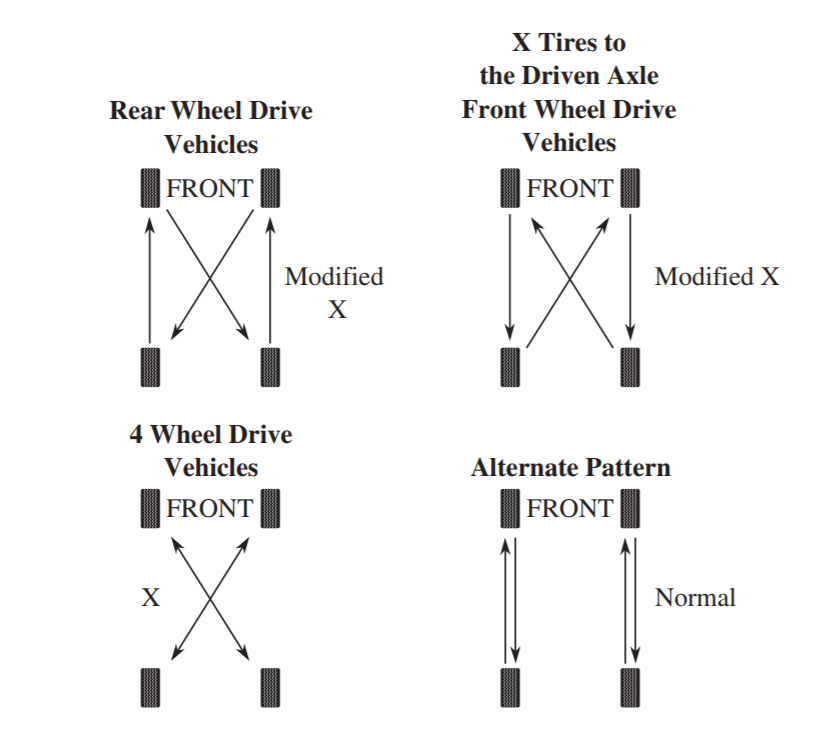
\includegraphics[scale=0.5]{tires1.png}}
\caption{tire arrangements}
\label{fig}
\end{figure}
First, number the tires as such
\begin{figure}[htbp]
\centerline{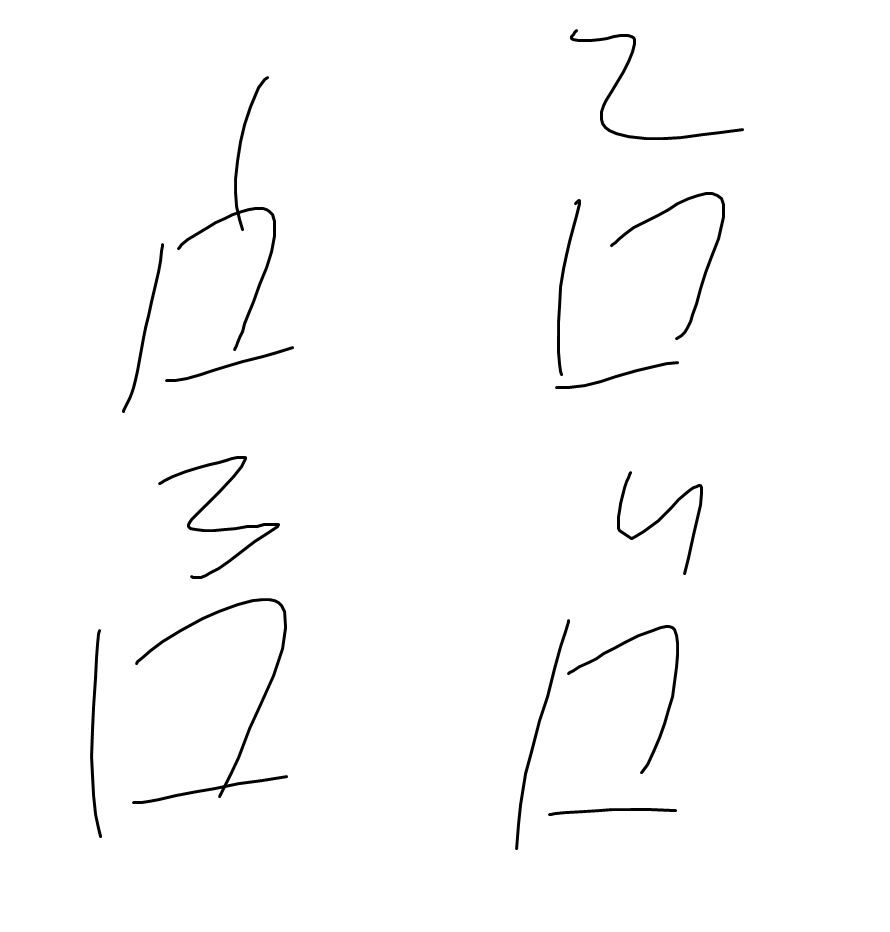
\includegraphics[scale=0.1]{tires.png}}
\caption{numbering}
\label{fig}
\end{figure}
Then the top-left arrangement can be described as a permutation that sends 1 to 4, 4 to 2, 2 to 3, and 3 back to 1. In cyclic notation, the top-left arrangement can be written $\alpha = (1423)$. Likewise, the top-right can be written $\beta = (1324)$, the bottom left $\gamma = (14)(23)$, and the bottom right $\sigma = (13)(24)$. For convenience, call the set of these four permutations $T$. \\

Clearly $T$ is not a subgroup of $S_4$, as it is not a group under function composition. There is no identity element. Nor is it closed. Take for example the composition $\gamma\sigma = (14)(23)(13)(24) = (12)(34)$. Clearly this is not an element of $T$. \\

How could we find the smallest subgroup of $S_4$ containing these elements? One method immediately jumps out. We could take every possible composition in $T$, and since this must be closed, and since each element in $T$ is also an element in $S_4$ which is a group, each element would also have an inverse. Since $S_4$ is finite, any subset of it must be finite, hence this knowledge would effectively prove that this is the smallest possible subgorup containing these elements. This, however, would not be fun (unless I made a program do it for me, which I might). There would be quite a few combinations to try (at least $4! = 24$), and whose to say that all 24 of them wouldn't be generated by the four elements in $T$. I really don't want to do it this way.\\
\fbox{solution} Consider the cylic subgroup formed by $\alpha$. Since $\alpha$ is a cycle of length 4, its has order $4$, and by a previously proven theorem about cyclic groups $|\alpha| =<\alpha> = \{\alpha,\alpha^2,\alpha^3,\epsilon\}$, where $\epsilon$ is the identity in both $<\alpha>$ and $S_4$. A quick computation of this reveals 

\\

\fbox{thought} What if I generalized the notion of a cycle. What I mean is that we have the idea of the group formed by $\alpha$ and $\beta$, and even of $\alpha\beta$, when we multiply this element by itself as many times as we want until it wraps itself back around (assuming that $\alpha$ is part of a finite group) We write $<\alpha> = \{\alpha,\alpha^2,\dots,\alpha^n\}$. Let $|\alpha| = m$ and $|\beta| = n$. What if to represent the set formed by all possible combinations of these elements, we wrote, $$<\alpha,\beta> = 
\{\alpha \beta, \alpha\beta^2, \dots,[\alpha\beta^m = \alpha],\alpha^2 \beta, \alpha^2\beta^2, \dots,[\alpha^2\beta^m = \alpha^2], \dots, [\alpha^n\beta = \beta],\dots,\beta^m\}.$$
What kinds of properties would this set have (under the same operation of the group which $\alpha,\beta$ are part of). I've heard the word "generator" said before, and I'm pretty this is what it is means. Just in case it isn't, let's use a different term. How about "seed" and set generated by the "seed."\\

\fbox{definition/theorem} Given a finite group $(G,*)$ and a nonempty subset of $G$, $S$, we call $<S>$ the seed of the subgroup of $G$ formed by the elements in $S$ under the group operation of $G$. \\
\fbox{proof that this is a subgroup}. Let $G$ be an arbitrary group and let $S\subseteq G$ be nonempty. Let $S$ by an arbitrary subgroup of $G$. Let $S = \{a_1,\dots,a_n\}$ for $a_1,\dots,a_n\in S$. Let $x,y\in <S>$. Then by definition of $S$, $x = a_1^{p_1}\dots a_n^{p_n}$ and $y = a_1^{q_1}\dots a_n^{q_n}$ for natural numbers $p_1,1_1,\dots,p_n,q_n$. Since $G$ is finite, and since $a_1,\dots,a_n \in G$, it follows that 
\end{document}